\problemname{Geimskip}
``A long time ago, in a galaxy far, far away\ldots''

Andspyrnuhreyfingin hefur loksins fundið staðsetningu nýju Death Star og hyggst
gera allsherjaráras undir stjórn Gial Ackbar flotaforingja. Ackbar hefur ræst
út allan flotann sem samanstendur af mismunandi skipum; MC80 stjörnuskipum,
CR90 korvettum, dornískum orustuskipum, YT-2400 létt freigátum og ýmsum minni
orustuþotum eins og T-65B X-vængjum.

Það sem Ackbar flotaforingi veit ekki er að Han Solo og teymi hans létust í
misheppnaðri tilraun til að eyðileggja orkustöðvar varnarskjaldarins. Að auki
hefur Piett aðmíráll sett upp gildru svo Keisaraveldið geti losað sig við
Andspyrnuhreyfinguna fyrir fullt og allt. Þessi vel útpælda gildra samanstendur
af sprengjum sem aðmírállinn hefur komið fyrir á þeim stað sem Andspyrnuflotinn
kemur úr ljóshraða.

Flugskip Andspyrnuflotans og sprengjur aðmírálsins koma í mismunandi stærðum og
til að einfalda hlutina getum við hugsað um þetta sem kúlur í þremur víddum. Ef
að sprengja hefur nógu stóran radíus til að skarast á við (eða snerta) flugskip
þá springur skipið. Þegar skip springur veldur það annarri sprengingu sem
samsvarar sprengju með tvöföldum radíus skipsins og getur þetta því valdið
keðjuverkun af sprengingum.

Þar sem Ackbar flotaforingi fékk vægt taugaáfall þegar hann uppgötvaði
gildruna, þá er hann ófær um að meta skaðann sem flotinn hlaut. Getur þú
hjálpað honum?


\section*{Inntak}
  Fyrsta lína inntaksins inniheldur eina heiltölu $N$. Á næstu $N$ línum eru
  lýsingar á geimskipum andspyrnuflotans þar sem $i$:ta línan inniheldur fjórar
  heiltölur $x_i,y_i,z_i$ og $r_i$. Fyrstu þrjár tölurnar $(x_i,y_i,z_i)$ tákna
  staðsetningu $i$:ta geimskipsins í þrívíðu rúmi og $r_i$ er radíus þess. Því
  næst kemur lína sem inniheldur eina heiltölu $M$. Á næstu $M$ línum eru
  lýsingar á sprengjum aðmírálsins þar sem $j$:ta línan inniheldur fjórar
  heiltölur $x_j,y_j,z_j$ og $r_j$. Fyrstu þrjár tölurnar $(x_j,y_j,z_j)$ tákna
  staðsetningu $j$:tu sprengjunnar í þrívíðu rúmi og $r_j$ er sprengiradíus hennar. Gera
  má ráð fyrir að engin tvö geimskip skarist.

\section*{Úttak}
  Prentið út eina heiltölu $k$, fjölda skipa andspyrnuflotans sem lifa gildruna af.

\section*{Útskýring á sýnidæmum}
  %\begin{wrapfigure}{l}{0.45\textwidth}
  \begin{figure}[h!]
    \centering
    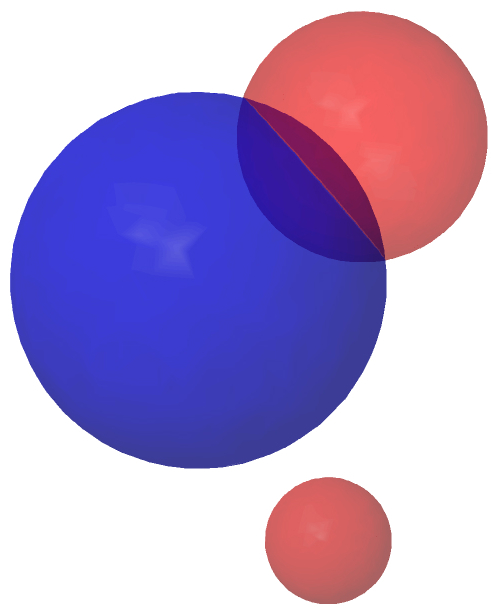
\includegraphics[width=0.3\textwidth]{zapped.jpg}
    \caption{\label{fig:bomb}Mynd af geimskipinu og sprengjunum tveimur úr sýnidæmi 1, táknuð sem kúlur í þrívíðu rúmi.}
  %\end{wrapfigure}
  \end{figure}

  Fyrsta sýnidæmið inniheldur eitt geimskip, staðsett í núllpunkti $(0,0,0)$ og
  með radíus $3$, og síðan tvær sprengjur. Fyrri sprengjan er staðsett í punktinum
  $(2,3,-3)$ og hefur sprengiradíus $1$. Seinni sprengjan er staðsett í $(-2,2,2)$
  og hefur radíus $2$. Eins og sést á myndinni þá hefur fyrri sprengjan
  engin áhrif á geimskipið en sú seinni er nógu öflug til að
  sprengja geimskipið. Því er úttakið $0$ þar sem ekkert geimskip lifði af.

  Í öðru sýnidæminu skarast engin skip og sprengjur og því lifir eina geimskipið af.

  Í síðasta sýnidæminu veldur fjórða sprengjan því að seinna geimskipið
  springur. Það hefur þau keðjuverkandi áhrif að fyrra skipið
  springur einnig. Ekkert skip lifir þetta af.

\section*{Stigagjöf}

\begin{tabular}{|l|l|l|l|}
\hline
Hópur & Stig & Inntaksstærð & Ónnur skilyrði \\ \hline
1 & 10 & $N = 1,\,0 \leq M \leq 10,\,-100 \leq x_i,y_i,z_i \leq 100,\,1 \leq r \leq 10$ & \\ \hline
2 & 10 & $N = 1,\,0 \leq M \leq 10^3,\,-100 \leq x_i,y_i,z_i \leq 100,\,1 \leq r \leq 10$ & \\ \hline
3 & 25 & $0 \leq N,M \leq 10^3,\,-100 \leq x_i,y_i,z_i \leq 100,\,1 \leq r \leq 10$ & Engar keðjuverkandi sprengingar\\ \hline
4 & 25 & $0 \leq N,M \leq 10^3,\,-100 \leq x_i,y_i,z_i \leq 100,\,1 \leq r \leq 10$ & \\ \hline
5 & 30 & $0 \leq N,M \leq 10^3,\,-10^4 \leq x_i,y_i,z_i \leq 10^4,\,1 \leq r \leq 10^3$ & \\ \hline
\end{tabular}

